\chapter{Introduction}\label{chap:introduction}


\section{Motivation and Outline}\label{sec:motivation-and-background}

Leaning-based methods and reinforcement learning have been succeeding in tasks of control complicated systems, for example robotic arms in \cite{levineEndtoEndTrainingDeep2016}.
However, one critical drawback of most of them is the lack of explicit and rigorous treatment of constraint satisfaction.
This significantly restricts their application in safety-critical scenarios, such as autonomous driving and racing.

A model-based predictive safety filter is proposed in \cite{wabersichLinearModelPredictive2018} for linear time invariant (LTI) systems, which can be used to ensure safety of the system under arbitrary objective inputs.
It is later extended to non-linear systems in \cite{wabersichPredictiveSafetyFilter2021a}.
It is successfully applied to the controlling of Chronos \cite{carronChronosCRSDesign2022}, a radio-controlled (RC) model vehicle, in \cite{tearlePredictiveSafetyFilterRacing2021}.
These proposed safety filters rely on a model of the system, which is used to predict future states and outputs of the system under proposed inputs.
Then the proposed safe inputs, which is close to the objective inputs, are applied to the system.
The system model typically comes from complicated modelling, possibly considering first principles, combined with a system identification procedure.
This process is almost always time-consuming, computationally expensive, and requires expert knowledge.
In this thesis we aim at designing a data-driven predictive safety filter, which only requires rich enough dataset trajectories of the system, instead of the system model.
The key idea is to skip the system identification process, and directly use dataset trajectories to predict future outputs of the system.

This idea of data-driven prediction is not new, and has been firstly developed in the context of noise-free LTI systems.
As introduced in \cite{willemsNotePersistencyExcitation2005}, the behavior of an LTI system can be fully captured by a rich enough dataset trajectory, which is commonly referred to as the \emph{fundamental lemma}.
Based on this fundamental lemma, the prediction of future outputs of a system can be achieved without the need of a model.
It firstly applied in the context of model predictive control (MPC), which also requires a model of the system to make predictions, and uses the predictions to tackle the control task directly \cite{garciaModelPredictiveControl1989}.
The combination of data-driven prediction and MPC is introduced in \cite{coulsonDataenabledPredictiveControl2019} in the name of \emph{Data-enabled predictive control (DeePC)}, where a dataset trajectory is directly used to predict future trajectories of the system.

This data-driven prediction method has also been extended to linear time invariant affine systems in \cite{martinelliDataDrivenAffine2022}, and to multiple dataset trajectories in \cite{vanwaardeMultiple2020}.
However, noise-free linear system is a very special case, and there are many challenges when extending the idea to more general systems, such as noisy linear systems and non-linear systems.

A scheme to deal with noise in both dataset trajectory and online observations is proposed in \cite{coulsonDataenabledPredictiveControl2019}: the regularization of auxiliary variables in the predictive controller.

Such DeePC controllers has been successfully applied in many fields.
For example in \cite{elokdaDataQuad2021}, DeePC is applied to the tracing problem of quadcopters.
A sensitivity analysis of hyperparameters in DeePC is also provided in \cite{elokdaDataQuad2021}, along with suggestions on how to choose them based on the empirical results.
DeePC is also used to model and control the noisy unknown dynamics of a quasi continuum manipulator in \cite{mullerDataDrivenQCR2022}.
The results show that DeePC can successfully deal with the noise and model discrepancy in the system, resulting in a dramatically reduced tracking error.
It is worth noticing that although the DeePC is originally designed for LTI systems, in \cite{elokdaDataQuad2021} and \cite{mullerDataDrivenQCR2022}, it is successfully applied to non-linear systems.

With the success of data-driven predictive control, it is natural to ask whether it is possible to design a data-driven predictive safety filter, which can be used to ensure safety of the system under arbitrary control inputs, and only requires dataset trajectories for off-line design.
Simultaneously to this thesis, a data-driven safety filter for noise-free LTI systems is proposed in \cite{bajelaniDataDrivenSafetyFilter2023}.
However, an extensive discussion of robust formulation and the, applicability to non-linear systems, and comparison of different formulations is yet to be done.
This thesis aims to fill this gap.

Apart from successful applications to real-world systems, a lot of effort has gone into showing theoretical guarantees of these data-driven methods, for example the comparison between \emph{Direct} and \emph{Indirect} methods in DeePC \cite{dorflerBridgingDirectIndirect2023}.
The direct method, as the name suggests, deals with the data trajectory directly, while the indirect method accepts a mild preprocessing of the dataset, similar to the method using instrumental variables in \cite{soderstromInstrumentalVariableMethods2002} and subspace identification in \cite{favoreelSPCSubspacePredictive1999}, which are shown to be equivalent in \cite{vanwingerdenInstrumentVar2022}.
It has been shown in \cite{dorflerBridgingDirectIndirect2023} that the regularized direct approach can be viewed as a convex relaxation of the indirect approach, and based on empirical results, the authors suggest indirect method in the case of variance errors such as output noise, and direct method in the case of bias errors such as model discrepancy.
In \cite{mattssonRegularizationDeePC}, different regularizers are proposed and compared, both in the context of DeePC and purely prediction problems.
The results reconfirm the conclusion in \cite{dorflerBridgingDirectIndirect2023}, that the indirect method outperforms direct method in the case of variance error.
In this thesis, we will also compare the direct and indirect methods, and show that the indirect method is better for safety filters, since it better decouples the prediction constraint and objective in optimization problem, therefore reduces unwanted input interference when the objective inputs are safe.

Similar to MPC, DeePC also faces the challenge of closed-loop guarantees, including recursive feasibility, constraint satisfaction and closed-loop stability.
Due to the lack of a model, relevant results are less mature compared to MPC.
In \cite{berberichDataDrivenRobust2021} and \cite{berberichStabilityInnerRobust2022IEEE}, qualitative guarantees have been proved for DeePC with mild modifications, namely with small enough noise bound, recursive feasibility and asymptotic stability hold in closed-loop.
The main drawback of these results is that no output constraints are considered.
In \cite{berberichRobustConstraintSatisfaction2020}, a constraint tightening scheme is proposed to ensure output constraints satisfaction in DeePC.
This scheme has the advantage of being rigorous, but the drawback is being conservative due to a generous estimation of prediction error.
In this thesis, we propose a less conservative, more realistic and flexible scheme of qualitative constraint tightening, and adopt the scheme proposed in \cite{berberichRobustConstraintSatisfaction2020} to prove qualitative guarantees of the proposed robust data-driven safety filter formulations.

There are also works for DeePC applied to non-linear systems.
In \cite{berberichLinearTrackingMPCData2022}, a data-driven predictive controller for non-linear systems is proposed, which can be used to track a reference trajectory.
The rationale is to linearize the system around current state, then applying DeePC to the linearized system.
Therefore, the dataset is updated at each time step with recent observations.
With mild assumptions, bound on the tracking error is established in \cite{berberichLinearTrackingMPCData2022}.
Simulation results show that the proposed controller can successfully track a reference trajectory.
This result relies on the assumption that the recent online observations are rich enough, and it lacks the ability to adapt to different system behaviors.
Also, it does not make use of possibly very rich off-line and historical dataset trajectories.
In this thesis, we propose another data-driven prediction scheme for non-linear systems, which is also based on local linearization, but takes advantage of rich off-line and historical dataset trajectories.

There are also works on a data-driven formulation that is different from DeePC, such as the one proposed in \cite{huangRobustDataEnabledPredictive2023}.
This scheme uses an auxiliary variable to take any possible error realization into account, and gives a tractable convex reformulation of the original problem.
Bound of open loop cost can be established, but the closed-loop guarantees and performance are yet to be discussed.
The possibility of applying this scheme to safety filter is left for future work.

The thesis is organized as follows.
We first give a brief introduction of the background, motivation and preliminaries in \cref{chap:introduction}.
Then we introduce the nominal data-driven safety filter in \cref{chap:nominal-ddsf}, and show that it is equivalent to the model-based safety filter for noise-free LTI system.
This equivalence is developed in parallel with the results in \cite{bajelaniDataDrivenSafetyFilter2023}.
As a result, theoretical guarantees including recursive feasibility and constraints satisfaction can be naturally established.
In \cref{chap:robust-ddsf-lti}, we incorporate the robust design methods into the proposed data-driven safety filter, resulting in two different formulations, one with direct method and rigorous constraint tightening and another with indirect method and qualitative tightening.
Numerical results also show that the proposed data-driven safety filter can successfully keep the system safe under arbitrary control inputs.
Comparison between the two formulations shows that indirect method is better for the safety filter, since it better decouples the prediction and input interfere, therefore reduces unwanted input interference when the objective inputs are safe.
Also, the qualitative constraint tightening scheme is less conservative and more flexible compared to the rigorous constraint tightening scheme.
In \cref{chap:non-linear-system}, we propose a data-driven prediction scheme for non-linear system, as well as a metric to evaluate the richness of datasets based on their fractal dimensions.
Numerical example using a simple two-dimensional non-linear system is given to show that the proposed data-driven prediction scheme yields more precise prediction compared to existing methods with rich enough dataset, and the metric is higher for richer dataset.
Finally, in \cref{chap:test-chronos}, we test the proposed data-driven safety filter on the simulation of Chronos \cite{carronChronosCRSDesign2022}, an RC model vehicle, and show that the safety filter can successfully keep the system safe under arbitrary control inputs.
We also propose and compare different terminal ingredient designs for the RC vehicle, as well as a practical dataset collection scheme for general systems.


\section{Preliminaries}\label{sec:preliminaries}

In this section, we introduce the notations, relevant background knowledge, definition and assumptions commonly used in this thesis.

The basic notations used in this thesis are list in \cref{tab:notations}.

{\renewcommand{\arraystretch}{1.5}
\vspace{0.1em}
\begin{center}
\captionof{table}{Basic notations. \label{tab:notations}}
\begin{tabular}{ c|l }
    $\listinI{i}{j}$ & List of integers from $i$ to $j$, $\left\{ i, i+1, \dots, j \right\}$ \\
    \hline
    $\listinIinf{i}$ & Infinite list of integers starting from $i$, $\left\{ i, i+1, i+2, \dots\right\}$ \\
    \hline
    $\sequence{x}{k}{i}{j}$ & A sequence of variables $\left\{ x_i, x_{i+1}, \dots, x_j \right\}$ \\
    \hline
    $\subseq{x}{i}{j}$ & Stack of a sequence of variables, usually vectors $\transpose{\begin{bmatrix}\transpose{x_i}, \transpose{x_{i+1}}, \cdots, \transpose{x_j}\end{bmatrix}}$ \\
    \hline
    $\norm{x}_P$ & $P$-norm of $x$, $\sqrt{\transpose{x} P x}$ \\
    \hline
    $A \otimes B$ & Kronecker product of real matrices $A$ and $B$ \\
    \hline
    $\Real^n$ & Set of real vectors of length $n$ \\
    \hline
    $\Real^{m \times n}$ & Set of $m$-by-$n$ real matrices \\
    \hline
    $\ones{n}$ & All one vector of length $n$ \\
    % \hline
    % $\text{diag}\left(a_1, a_2, a_3, \cdots\right)$ & Diagonal matrix with diagonal elements $a_1, a_2, a_3, \cdots$ \\
    \hline
    $\Xset \times \Yset$ & Cartesian product of sets $\Xset$ and $\Yset$ \\
    \hline
    $\Xset^N$ & Cartesian product of $N$ copies of $\Xset$ \\
\end{tabular}
\end{center}
}

With a little abuse of notation, we use $x$ to denote a sequence $\sequence{x}{k}{i}{j}$ if the index range $i$ and $j$ are clear from the context.
This usually occurs when we are defining the variables of an optimization problem, and the index range is clear from the objective and constraints of it.
We also accept the fact $\RealVec{n} \times \RealVec{m} = \RealVec{n+m}$, and similarly $\Xset \times \Yset \subseteq \RealVec{n+m}$ if $\Xset \subseteq \RealVec{n}$ and $\Yset \subseteq \RealVec{m}$.

In this thesis we extensively discuss optimization problems.
We use variables without accents to denote online observation and closed loop response.
Subscripts are used to denote time steps, for example $x_t$ denotes the state of the system at time step $t$.
And we use different accents to denote different types of variables, as shown in \cref{tab:opt-accents}.
In the table $a$ is just a dummy variable to show the accents.

{\renewcommand{\arraystretch}{1.5}%
\vspace{0.1em}
\begin{center}
\captionof{table}{Accents for variables. \label{tab:opt-accents}}
\begin{tabular}{ c|l }
    $\bar{a}$ & Optimization variables \\
    \hline
    $a^*$ & Optimal solution \\
    \hline
    $\hat{a}$ & Candidate solution \\
    \hline
    $\tilde{a}$ & Data or online observation with noise \\
    \hline
    $\check{a}$ & \parbox{0.7\textwidth}{Real system state/output without noise if the proposed control input sequence is applied} \\
\end{tabular}
\end{center}
}

When it is necessary, we also use brackets to denote the time step of the optimization problem, for example $\barx(t)$ represents the optimization variable for  the system state at time step $t$, and $\hatx(t+1)$ represents a candidate solution for time step $t+1$.

Without further notice, we always deal with discrete time invariant systems.

\begin{definition}[Discrete time invariant dynamic system]\label{def:dynamic-system}
    A discrete time invariant dynamic system is defined by $\left(\Xset, \Uset, \Yset, f, g\right)$, where:
    $\Xset \subseteq \Real^n$ is the state constraint set;
    $\Uset \subseteq \Real^m$ is the input constraint set;
    $\Yset \subseteq \Real^p$ is the output constraint set;
    $f: \Real^n \times \Real^m \rightarrow \Real^n$ is a function representing system dynamics;
    $g: \Real^n \times \Real^m \rightarrow \Real^p$ is the output function.
\end{definition}

For the rest of the thesis, without further notice, we always assume the dimension of state, input and output are $n$, $m$ and $p$ respectively.

Note that we define the functions $f$ and $g$ on the ambient linear space $\Real^n$ and $\Real^m$, instead of the constraint sets $\Xset$ and $\Uset$.
This is for the convenience of discussing \emph{trajectories} and \emph{safe trajectories} of the system, where a trajectory is a list of input-output pairs that satisfy the system dynamics but can violate the constraints.

\begin{definition}[Trajectory of a dynamic system]\label{def:traj-dynamical-system}
    A list of input-output pairs $\sequence{u}{t}{i}{j}$ and $\sequence{y}{t}{i}{j}$, with $u_t \in \Real^m$ and $y_t \in \Real^p$, is called a trajectory of the dynamic system $\left(\Xset, \Uset, \Yset, f, g\right)$ if there exist $\sequence{x}{t}{i}{j}$, $x_t \in \Real^n$, with $x_t = f\left(x_{t-1}, u_{t-1}\right)$, and $y_t = g\left(x_t, u_t\right)$ hold for any $t$ in $\listinI{i+1}{j}$.
\end{definition}

\begin{remark}\label{remark:state-unique}
    Depending on properties of $f$ and $g$, It is not necessary true that the state $x_t$ is uniquely determined by the one input-output pair $\left(u_t, y_t\right)$.
    It is possible that we need more than one input-output pairs to uniquely determine the state of the system, or even impossible to uniquely determine the state of the system with finite input-output pairs.
\end{remark}

As for a safe trajectory, it is a trajectory that can be extended into an infinite trajectory of the system, and keep the constraints satisfied for all time steps.

\begin{definition}[Safe trajectory of a dynamic system]\label{def:safe-traj}
    A list of input-output pairs $\sequence{u}{t}{i}{j}$ and $\sequence{y}{t}{i}{j}$, with $u_k \in \Real^m$ and $y_t \in \Real^p$, is called a safe trajectory of the dynamic system $\left(\Xset, \Uset, \Yset, f, g\right)$, if there exist $\sequence{\hatu}{t}{i}{\infty}$, $\sequence{\hatx}{t}{i}{\infty}$, and $\sequence{\haty}{t}{i}{\infty}$ that satisfy the following conditions:
    {
    \setlength{\topsep}{0pt}
    \setlength{\parskip}{0pt}
    \begin{enumerate}
        \item $\hatx_{t+1} = f\left(\hatx_t, \hatu_t\right)$, $\haty_t = g\left(\hatx_t, \hatu_t\right)$ hold for any $t$ in $\listinIinf{i}$.
        \item $\hatx_t \in \Xset$, $\hatu_t \in \Uset$, $\haty_t \in \Yset$ hold for any $t$ in $\listinIinf{i}$.
        \item $\hatu_t = u_t$, $\tildey_t = y_t$ hold for any $t$ in $\listinI{i}{j}$.
    \end{enumerate}
    }
\end{definition}

\begin{remark}\label{remark:safe-traj}
    As discussed in \cref{remark:state-unique}, it is only possible to uniquely determine the state of the system with a long enough input-output trajectory, for some certain systems.
    % For example, the trajectory needs to be at least of length $l$ in the case of LTI system.
    But a shorter trajectory that can not determine the state of the system can still be safe, according to \cref{def:safe-traj}.
    In this case, the fact that \emph{online observation over a time span $t_1$ to $t_2$ forms a safe trajectory} does not imply that \emph{the system can be kept safe for all future time steps after $t_2$}.
    Whether the system can be kept safe after $t_2$ ultimately depends on the state of the system at $t_2$.
    % This implication only holds if, the online observation from $t_1$ to $t_2$ is long and rich enough to uniquely determine the state of the system.
\end{remark}

Within the scope of this thesis, we assume that the system state is not constrained.

\begin{assumption}\label{asm:no-state-constraint}
    The state of the system is not constrained, that is $\Xset = \Real^n$.
\end{assumption}

As common in system theory, a time invariant dynamic system is linear if both the state transition function $f$ and output function $g$ are linear and can be represented by matrices.

\begin{definition}[Linear time invariant system]\label{def:lti-system}
    A dynamic system $\left(\Xset, \Uset, \Yset, f, g\right)$ is called linear time invariant (LTI) if both $f$ and $g$ are linear functions.
    Equivalently, they can be represented by matrices $A \in \RealMat{n}{n}$, $B \in \RealMat{n}{m}$, $C \in \RealMat{p}{n}$, $D \in \RealMat{p}{m}$ as: $f\left(x,u\right) = A x + B u$, $g\left(x, u\right) = C x + D u$.
    We also use $\ltimatrices$ to denote the dynamic of an LTI system, since it captures all the information of functions $f$ and $g$.
\end{definition}

A slightly more complicated family of systems is affine systems, where $f$ and $g$ are affine functions.

\begin{definition}[Affine system]\label{def:affine-system}
    A dynamic system $\left(\Xset, \Uset, \Yset, f, g\right)$ is called affine if both $f$ and $g$ are affine functions.
    Equivalently, they can be represented by matrices $A \in \RealMat{n}{n}$, $B \in \RealMat{n}{m}$, $C \in \RealMat{p}{n}$, $D \in \RealMat{p}{m}$ and vectors $a_f \in \RealVec{n}$, $a_g \in \RealVec{m}$ as: $f\left(x,u\right) = A x + B u + a_f$, $g\left(x, u\right) = C x + D u + a_g$.
\end{definition}

In \cref{chap:nominal-ddsf,chap:robust-ddsf-lti}, we deal with LTI systems.
While in \cref{chap:non-linear-system}, we touch upon affine systems and non-linear systems.

By \emph{Kalman Decomposition} \cite{kalmanMathematicalDescriptionLinear1963}, any LTI system can be decomposed to observable/unobservable and controllable/uncontrollable parts.

For simplicity, we define the controllability of an LTI system as the controllability of the pair of matrices $A$ and $B$:

\begin{definition}[Controllability of LTI systems]\label{def:lti-controllability}
    A pair of dynamic matrices $A$ and $B$ is controllable, if the controllability matrix $\mathcal{C}_n = \begin{bmatrix} B & A B & \ldots & A^{n-1} B \end{bmatrix}$ has full row rank.
    Where $n$ is the dimension of the state of the system.
\end{definition}

% As a reference to behavior system theory discussed in \cite{markovskyBehavioralSystemsTheory2021}, different dynamic matrices may give the same input-output response behavior $\mathscr{B}$.
% Also, a certain behavior $\mathscr{B}$ can also be controllable or not.
Different matrices pairs like $(A, B, C, D)$ and $\left(A', B', C', D'\right)$, may result in the same input-output response behavior.
This is captured by the concept of \emph{behavior} in behavioral system theory \cite{markovskyBehavioralSystemsTheory2021}.
Within this scope of this thesis, we use the following definition of ``having the same behavior''.

\begin{definition}[LTI systems with same behavior]\label{def:lit-same-behavior}
    Two LTI systems with system dynamics $\ltimatrices$ and $\left(A', B', C', D'\right)$ have the same behavior, if any trajectory of the first system is also a trajectory of the second system, and vice versa.
\end{definition}

It is possible that two LTI systems have the same behavior, but the dimension of the state of the two systems are different.
In this thesis we focus on the input-output behavior of the system, and we don't deal with state constrains, so we work with minimal realizations \cite{markovskyBehavioralSystemsTheory2021} to avoid this complexity.

\begin{definition}[Minimal realization]\label{def:lti-minimal-realization}
    An LTI system with system dynamics $\ltimatrices$ is called minimal realization, if the dimension $n$ of its state space is the smallest among all LTI systems with the same behavior.
\end{definition}

\begin{remark}\label{remark:observability-minimal}
    It follows from Kalman Decomposition \cite{kalmanMathematicalDescriptionLinear1963} that omitting the unobservable part of a system will result in a system with same behavior.
    So by \cref{def:lti-minimal-realization} we can conclude that a minimal realization is always observable.
\end{remark}

\begin{assumption}\label{asm:lti-minimal-realization}
    We always assume the LTI system with system dynamics $\ltimatrices$ is a minimal realization.
\end{assumption}

Then we can define the order and lag of LTI systems with same behavior.

\begin{definition}[Order and lag of LTI system]\label{def:order-lag}
    For a family of LTI systems with same behavior, suppose we have a minimal realization $\ltimatrices$.
    We define the order $n$ as the dimension of the state under this minimal realization.
    And we define lag of the system as the minimal integer $l$, that makes the observability matrix $\Phi_l = \transpose{\begin{bmatrix} \transpose{C} & \transpose{(C A)} & \ldots & \transpose{(C A^{l-1})} \end{bmatrix}}$ of full rank.
    For simplicity, we also use the term ``order and lag of the system'' to refer to the order and lag of the the family of systems with same behavior.
\end{definition}

\begin{remark}\label{remark:order-lag}
    Note that for a family of LTI systems with same behavior, the order and lag are well-defined, independent of the minimal realization, and $l \leq n$ holds \cite{markovskyBehavioralSystemsTheory2021}.
    Also, the lag $l$ is the minimal number of input-output pairs needed to uniquely determine the state of the system \cite{markovskyBehavioralSystemsTheory2021}.
\end{remark}

It follows from \cref{remark:order-lag} that we can uniquely determine the state of an observable LTI system with a dataset trajectory of length $l$ or larger.
We can then define the \emph{Extended State} for an observable LTI system.

\begin{definition}[Extended state]\label{def:extedned-state}
    We call a trajectory of length larger than $l$ the extended state of an observable LTI system.
    The notation $\zeta_t = \extendedstateinline{t-n}{t-1}$ and $\xi_t = \extendedstateinline{t-l}{t-1}$ will be used to denote these extended states with specific length.
\end{definition}

With the above definitions and assumptions, we can try to deal with the problem of data-driven prediction:
how can we make predictions of future outputs of the system, if we only have a dataset trajectory, online observation, and proposed control inputs?
To tackle this problem, we need to introduce more concepts.

The \emph{Hankel matrix} of certain depth constructed with a sequence of vectors is defined as:

\begin{definition}[Hankel matrix]\label{def:hankel-matrix}
    For a sequence of vectors $\sequence{x}{k}{i}{j}$, with $x_k \in \Real^n$, the Hankel matrix of depth $L$ is defined as:
    \begin{equation*}
        \hankel{L}{\sequence{x}{k}{i}{j}} = \begin{bmatrix}
            x_i & x_{i+1} & \ldots & x_{j-L+1} \\
            x_{i+1} & x_{i+2} & \ldots & x_{j-L+2} \\
            \vdots & \vdots & \ddots & \vdots \\
            x_{i+L-1} & x_{i+L} & \ldots & x_{j}
        \end{bmatrix} \in \RealMat{(n \times L)}{(j-i-L+2)} \textstop
    \end{equation*}

\end{definition}

Each column of the Hankel matrix is the vertical stack of a sub-sequence with length $L$ of the original sequence. 
And all columns cover all possible length-$L$ sub-sequences of the original sequence.
Suppose we have a sequence of inputs $\sequence{u}{t}{i}{j}$, then the Hankel matrix $\hankel{L}{\sequence{u}{t}{i}{j}}$ can be constructed by taking a ``window'' of length $L$ and slide it along the sequence, and stack all the windows vertically.

The \emph{fundamental lemma} of data-driven predictive control, as introduced in \cite{willemsNotePersistencyExcitation2005}, states that the behavior of an LTI system can be fully captured by a \emph{rich enough} dataset trajectory.
Here rich enough is formally captured by the definition of \emph{persistently exciting} dataset trajectory:

\begin{definition}[Persistently exciting]\label{def:persistently-exciting}
    We say a sequence of inputs $\sequence{u}{k}{0}{N-1}$ is persistently exciting of order $L$, if the Hankel matrix $\hankel{L}{\sequence{u}{k}{0}{N-1}}$ has full row rank (of rank $m \times L$).
\end{definition}

% And the assumption we need for the dataset trajectory is also related to the system order.

% \begin{assumption}\label{asm:persistently-exciting}
%     The input sequence to an LTI system $\sequence{u}{k}{0}{N-1}$ is persistently exciting of order $L + n$, where $n$ is the order of the minimal realization with same behavior of the system.
% \end{assumption}

Then we can state the fundamental lemma as:

\begin{lemma}[Fundamental lemma]\label{lemma:fundamental-lemma}
    Consider a controllable LTI system and a dataset trajectory $\datasetSequence{u}{N}$ and $\datasetSequence{y}{N}$ of the system.
    If $\datasetSequence{u}{N}$ is persistently exciting of order $L+n$, then $\sequence{u}{t}{0}{L-1}$ and $\sequence{y}{t}{0}{1}$ form a trajectory of the system if and only if there exist $\alpha \in \RealVec{N-L+1}$, which makes the following equation hold:
    \begin{equation*}
        \begin{bmatrix}
            \subseq{u}{0}{L-1} \\
            \subseq{y}{0}{L-1} \\
        \end{bmatrix} = \begin{bmatrix}
            \hankel{L}{\datasetSequence{u}{N}} \\
            \hankel{L}{\datasetSequence{y}{N}} \\
        \end{bmatrix} \alpha \textstop
    \end{equation*}
\end{lemma}

\Cref{lemma:fundamental-lemma} states that a rich enough dataset trajectory can represent the system behavior up to a certain length, so it shows the possibility of replacing a model of the system with only a dataset trajectory.

Also, as mentioned in \cref{remark:order-lag}, it is possible to uniquely determine the state of the system with a dataset trajectory of length that is larger than $l$.
By this intuition, we can define the input-output equilibrium of the system:

\begin{definition}[Input-output equilibrium]\label{def:input-output-equilibrium}
    An input-output pair $\left(\us, \ys\right)$ is called an input-output equilibrium of an observable LTI system, if $\left\{\us\right\}_{t=0}^{l}$ and $\left\{\ys\right\}_{t=0}^{l}$ is a trajectory of the system.
    Where $l$ is the lag of the LTI system.
\end{definition}

The intuition is that, if a pair $\left(\us, \ys\right)$ satisfies \cref{def:input-output-equilibrium}, then $\left\{\us\right\}_{t=0}^{\infty}$ and $\left\{\ys\right\}_{t=0}^{\infty}$ is a trajectory of the system.
Which means the system can stay at the input-output equilibrium forever.
Also, there will be an induced equilibrium state $\xs$, which is uniquely determined by $\left(\us, \ys\right)$, as discussed in \cref{remark:order-lag}.
It also satisfies $\xs = A \xs + B \us$ and $\ys = C \xs + D \us$ as a consequence of \cref{def:traj-dynamical-system,def:input-output-equilibrium}, so $\xs$ can be obtained given $\us$ and $\ys$ by solving the following equation:
\begin{equation}\label{eq:equilibrium-state}
    \begin{bmatrix}
        \xs \\
        \ys
    \end{bmatrix} = \begin{bmatrix}
        A & B \\
        C & D
    \end{bmatrix} \begin{bmatrix}
        \xs \\
        \us
    \end{bmatrix} \textstop
\end{equation}

\begin{definition}[Safe equilibrium]\label{def:safe-input-output-equilibrium}
    We call an input-output equilibrium $\left(\us, \ys\right)$ of an LTI system safe, if $\us \in \Uset$ and $\ys \in \Yset$ hold.
    This pair also implicitly induces a safe equilibrium state $\xs$.
\end{definition}

\begin{remark}\label{remark:safe-equilibrium}
    According to \cref{def:safe-traj}, if $\left(\us, \ys\right)$ is a safe input-output equilibrium of the system, then $\constantSequence{\us}{0}{L-1}$ and $\constantSequence{\ys}{0}{L-1}$ is also a safe trajectory for the system with any length $L$.
\end{remark}

In practice, we always need to deal with noisy data and noisy system dynamics.
Within the scope of this thesis, we only deal with additive, bounded output noise.

\begin{definition}[Additive output noise]\label{def:output-noise}
    A dynamic system with additive output noise is a dynamic system $(\Xset, \Uset, \Yset, f, g)$, where we can only observe the output with noise, that is $\tildey_t = g(x_t, u_t) + \varepsilon_t$, where $\varepsilon_t \in \Real^p$ is the output noise at time step $t$.
\end{definition}

In \cref{chap:robust-ddsf-lti} and \cref{chap:test-chronos}, we discuss different bounds of the noise.

Finally, we give a brief introduction to predictive safety filter, as introduced in \cite{wabersichLinearModelPredictive2018} and \cite{wabersichPredictiveSafetyFilter2021a}.
As already mentioned in \cref{sec:motivation-and-background}, predictive safety filter aims at keeping the system safe under arbitrary control inputs.
For now let's assume we have full observation of the system, which means $g(x,u) = x$.
With a general leaning based controller $\pi_l$, which can give any inputs, the overall data flow can be seen in \cref{img:predictive-safety-filter}.
A safety filter is attached to the system, which takes input from the learning based controller, the state of the system, and gives out a safe input to the system.

\begin{figure}[ht]
    \centering
    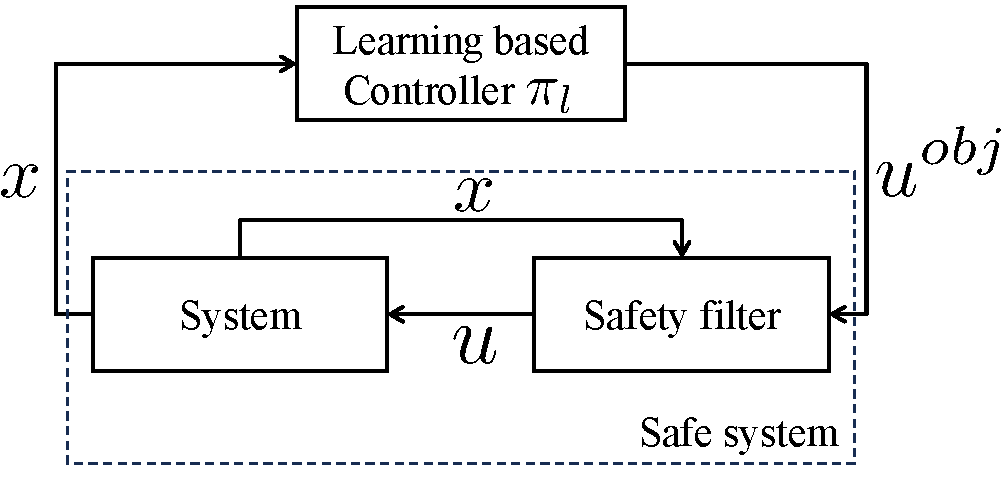
\includegraphics[width=0.7\textwidth]{\imagedir/predictiveSF.pdf}
    \caption{Illustration of predictive safety filter.}
    \label{img:predictive-safety-filter}
\end{figure}

With a dynamic system $\left(\Xset = \RealVec{n}, \Uset, \Yset, f, g(x,u) = x\right)$, the predictive safety filter solves the following optimization problem:
\begin{subequations}
\label{eq:state-based-safety-filter} 
\begin{align}
    \min_{\substack{\bar{u}, \bar{x}}} \quad & \norm{u_{0} - u^{\text{obj}}(t)}_R  \label{eq:state-based-safety-filter-cost} \\
    \textrm{s.t.} \quad & 
    \bar{x}_{k} = f(\barx_{k-1}, \baru_{k-1}) \quad k \in \left[1, L-1\right] \label{eq:state-based-safety-filter-dynamics} \\
    & 
    \barx_0 = x_t \label{eq:state-based-safety-filter-initial}\\
    & 
    \barx_{L-1} \in \Sset_f \label{eq:state-based-safety-filter-terminal} \\
    &
    \bar{u}_k \in \Uset, \quad k \in \left[0, L-1\right] \label{eq:state-based-safety-filter-input}\\
    &
    \bar{x}_k \in \Xset, \quad k \in \left[0, L-1\right] \textperiod \label{eq:state-based-safety-filter-output}
\end{align}
\end{subequations}
where $L$ is the prediction horizon, $x_t$ is the current state of the system, $\uObj(t)$ is current control input supposed by the learning based controller$\pi_l$, $R$ is the weighting matrix used to examine the distance between the actual input and the desired input.

$\Sset_f$ is a safe terminal set of the system, modified from Assumption 4.2 in \cite{wabersichPredictiveSafetyFilter2021a}.

\begin{definition}[Safe terminal set]\label{def:safe-terminal-state}
    $\Sset_f \subseteq \Yset$ is a safe terminal set of the system $(\Xset = \RealVec{n}, \Uset, \Yset \subseteq \RealVec{n}, f, g(x,u) = x)$, if the following holds: there exists a safe terminal controller $\pi_f: \Sset_f \to \Uset$, which makes $f(x, \pi_f(x)) \in \Sset_f$ hold for all $x \in \Sset_f$. 
\end{definition}

Intuitively, it is a set of states, so that there exists a safe terminal controller, which can keep the system within this set for all future time steps if the system starts from this set.

For predictive controllers, it is common to use \emph{one-step receding horizon} scheme.
This means at each time step the optimization problem is solved, and only the first input of the optimal solution is applied to the system.
Then the optimization problem is solved again at the next time step, with the new state of the system and the new desired input.
For the robustness of data-driven predictive controllers and safety filters, we need to introduce a slightly different \emph{multi-step receding horizon} scheme, as discussed in \cite{berberichDataDrivenRobust2021}.

\begin{definition}[Multi-step receiding horizon scheme]\label{def:multi-step-receding-horizon}
    For a predictive controller or safety filter, we say it is working under k-step receding horizon scheme, if at certain time step $t$, the optimization problem is solved with online observation and possibly some additional inputs, and only the first $k$ input of the optimal solution $\sequence{\staru}{i}{0}{k-1}(t)$ is applied to the system.
    Then at time step $t+k$, the optimization problem is solved again with the new online observations and additional inputs.
\end{definition}

We also have the following definition of recursive feasibility and close loop constraint satisfaction for multi-step receding horizon scheme.

\begin{definition}[Recursive feasibility]\label{def:recursive-feasibility}
    A predictive controller or safety filter with the form of an optimization problem is recursively feasible under k-step receding horizon scheme, if the following holds: if the optimization problem is feasible at time step $t$, then the optimization problem will be feasible also at time step $t+k$.
\end{definition}

\begin{definition}[Closed-loop constraint satisfaction]\label{def:closed-loop-constraint-satisfaction}
    A predictive safety filter provides constraint satisfaction in closed-loop under k-step receding horizon scheme, if the following holds: if the optimization problem is feasible at time step $t$, then after the input sequence $\sequence{\staru}{i}{0}{k-1}(t)$ is applied to the system, the outputs $\sequence{y}{i}{t}{t+k-1}$ stay in output constraint $\Yset$.
\end{definition}

\begin{remark}\label{remark:recursive-feasibility}
    It follows from \cref{def:recursive-feasibility,def:closed-loop-constraint-satisfaction} that: if both recursive feasibility and closed-loop constraint satisfaction hold for a predictive safety filter, and at the time step $t_0$ the optimization problem is feasible, then the system equipped with it is safe under arbitrary control inputs at all time steps $t \geq t_0$.
\end{remark}

As discussed in \cite{wabersichPredictiveSafetyFilter2021a}, recursive feasibility and closed-loop constraint satisfaction can be proven for this safety filter, following the one-step receding horizon scheme.
% In another word, if the optimization problem is feasible at time step $0$, then the constraint will be satisfied and the optimization problem will be feasible at all future time steps $t \geq 0$.
